% 
\usepackage{mathpartir}

\usepackage{graphicx}

% \usepackage[firstpage]{draftwatermark}
% % \SetWatermarkText{\hspace*{8in}\raisebox{3.5in}{\includegraphics[scale=0.1]{aec-badge-popl.pdf}}}
% \SetWatermarkText{\hspace*{13.3in}\raisebox{-6.5in}{\includegraphics[scale=0.1]{aec-badge-popl.pdf}}}
% \SetWatermarkAngle{0}

%--------------------------------------
% To use \mathbb
\usepackage{amsfonts}
%--------------------------------------
% To defined theorems and Lemmas
 \usepackage{amsthm} 
\theoremstyle{definition}  % non-italic
% Definition, Lemma and Theorem
\newtheorem{definition}{Definition}
\newtheorem{theorem}{Theorem}
% \newtheorem{definition}{Lemma}
\newtheorem{lemma}{Lemma}
\newtheorem{corollary}{Corollary}
%--------------------------------------
% To have colored annotations
\usepackage{xcolor}
%--------------------------------------
% To strike out text
\usepackage[normalem]{ulem}
\usepackage{cancel}
%--------------------------------------
%\usepackage{hyperref}
\usepackage{url}
%--------------------------------------
% Programming language rules
\usepackage{mmm}
\usepackage{pl}
%--------------------------------------
% Arrow symbols 
\let\Bbbk\relax
\usepackage{amssymb}
%--------------------------------------
% \xrightarrow
\usepackage{amsmath}
%--------------------------------------
% % To write algorithms
% \usepackage{algorithm}
% %\usepackage{algpseudocode}
% \usepackage[noend]{algpseudocode}
% \let\algState\State
% \usepackage{varwidth}% http://ctan.org/pkg/varwidth
% % To have Algorithm float
% % \usepackage{algorithm}
% % To make the algorithms float to the top
% \usepackage{float}
% \newfloat{algorithm}{t}{lop}
% %\renewcommand{\algorithmicforall}{\textbf{foreach}}
%--------------------------------------

% this employs smarter hyphenations, par, and other rules
% ... and helps condense the paper
\usepackage{microtype}

% To remove a warning for fonts
% \usepackage{lmodern}% http://ctan.org/pkg/lm

%--------------------------------------
% Symbol definitions and comments
% Standard
\def\t{\phantom{X}}

\def\<{\langle}
\def\>{\rangle}

%--------------------------------------

\usepackage{listings}
\lstset{
   language=C,
   captionpos=b,
   tabsize=3,
%   frame=lines,
%   keywordstyle=\color{blue},
%   commentstyle=\color{darkgreen},
%   stringstyle=\color{red},
   numbers=left,
   numberstyle=\tiny,
   numbersep=5pt,
   breaklines=true,
   showstringspaces=false,
%   basicstyle=\small\bfseries,
   basicstyle=\small\ttfamily,
   emph={label}
}

\usepackage{array}

\usepackage{tikz}
\usetikzlibrary{positioning} 
\usetikzlibrary{arrows} 
%\usetikzlibrary{graphs} % Not supported by tikz 2.10
\usetikzlibrary{calc}
\usetikzlibrary{backgrounds}
\usetikzlibrary{shapes}

%\usepackage{caption}
%\usepackage{subcaption}

\usepackage{stmaryrd}

\def\defeq{\triangleq}

\def\self{\mathit{self}}

\def\switch{\mathsf{switch} \ }
\def\case{\mathsf{case} \ }
\def\ret{\mathsf{ret} \ }
\def\lforall{\mathsf{forall} \ }
\def\lif{\mathsf{if} \ }
\def\lelse{\mathsf{else} \ }
\def\lmap{\mathsf{map} \ }
\def\llet{\mathsf{let} \ }
\def\max{\mathsf{max}}

\def\vc{\mathit{vc}}
\def\List{\mathsf{List}}
\def\llookup{\mathsf{lookup} \ }

\def\RYW{\mathit{RYW}}
\def\MR{\mathit{MR}}
\def\WFR{\mathit{WFR}}
\def\MW{\mathit{MW}}
\def\CC{\mathit{CC}}
\def\LCC{\mathit{LCC}}
\def\Rel{\mathit{Rel}}

\def\ext{\mathsf{ext}}

\def\CState{\mathsf{CState}}
\def\RState{\mathsf{RState}}

\def\true{\mathsf{true}}
\def\Set{\mathsf{Set}}
\def\Nat{\mathsf{Nat}}
% \def\L{\mathsf{L}}
\def\L{L}
\def\lab{\mathit{label}}
\def\clientLabs{\mathit{client\text{-}labels}}

\def\cInit{\mathsf{c\text{-}init}}
\def\rInit{\mathsf{r\text{-}init}}

\def\get{\mathsf{get}}
\def\getGuard{\mathsf{get\text{-}guard}}
\def\getReq{\mathsf{get\text{-}req}}
\def\getRes{\mathsf{get\text{-}res}}

\def\lput{\mathsf{put}}
\def\putGuard{\mathsf{put\text{-}guard}}
\def\putReq{\mathsf{put\text{-}req}}
\def\putRes{\mathsf{put\text{-}res}}

\def\Type{\mathsf{Type}}
\def\Option{\mathsf{Option}}
\def\Bool{\mathsf{Bool}}

\def\Event{\mathit{Event}}
\def\Req{\mathit{Req}}
\def\req{\mathit{req}}

\def\Res{\mathit{Res}}
\def\res{\mathit{res}}

\def\PutReq{\mathit{Put\text{-}req}}
\def\PutReqPayload{\mathsf{Put\text{-}req\text{-}payload}}
\def\PutRes{\mathit{Put\text{-}res}}
\def\PutResPayload{\mathsf{Put\text{-}res\text{-}payload}}

\def\GetReq{\mathit{Get\text{-}req}}
\def\GetReqPayload{\mathsf{Get\text{-}req\text{-}payload}}
\def\GetRes{\mathit{Get\text{-}res}}
\def\GetResPayload{\mathsf{Get\text{-}res\text{-}payload}}

\def\Unit{\mathsf{Unit}}

% Program Syntax

% Uses:
% $
% \sPut{}{},
% \sPut{k}{v},
% \sPut[i]{k}{v},
% % 
% \sGet{}{},
% \sGet{x}{k},
% \sGet[i]{x}{k},
% $

\newcommand\sPut[3][]{%
  \mathit{put}%
  \ifthenelse{\equal{#1}{}}{%
    \ifthenelse{\equal{#2}{}}{}{
    ({#2},{#3})}%
  }{%
    ^{#1}({#2},{#3})%
  }%
}  
  
\newcommand\sGet[3][]{%
   \ifthenelse{\equal{#2}{}}{}{#2\leftarrow}%
   \mathit{get}
   \ifthenelse{\equal{#1}{}}{}{^{#1}}%
   \ifthenelse{\equal{#3}{}}{}{({#3})}}

% \newcommand\sGet[2][]{%
%     \ifthenelse{\equal{#1}{}}{}{#1\leftarrow }%
%     \mathit{get}%
%     \ifthenelse{\equal{#2}{}}{}{({#2})}}
    
  \newcommand\sSkip{\mathit{skip}}

\newcommand{\name}[1]{\textsc{#1}}

\newcommand\indrule[3][]{%
%  \inferrule*[Right=#1]{#2}{#3}%
  \inferrule[#1]{#2}{#3}%
  }

\newcommand\figurealgtextsize{%
%   \small%
  \setlength{\abovedisplayskip}{0pt}%
  \setlength{\abovedisplayshortskip}{0pt}%
  \setlength{\belowdisplayskip}{0pt}%
  \setlength{\belowdisplayshortskip}{0pt}}
\newcommand\figureruletextsize{%
%   \small
  \setlength{\abovedisplayskip}{0pt}%
  \setlength{\abovedisplayshortskip}{0pt}%
  \setlength{\belowdisplayskip}{0pt}%
  \setlength{\belowdisplayshortskip}{0pt}
}
\newcommand\figuredefstextsize{%
%   \small
%  \large  
  \setlength{\abovedisplayskip}{0pt}%
  \setlength{\abovedisplayshortskip}{0pt}%
  \setlength{\belowdisplayskip}{0pt}%
  \setlength{\belowdisplayshortskip}{0pt}
}

\usepackage{siunitx}  % To format numbers

\setlength{\textfloatsep}{20pt}

\usepackage{balance}

% \newfont{\mycrnotice}{ptmr8t at 7pt}
% \newfont{\myconfname}{ptmri8t at 7pt}
% \let\crnotice\mycrnotice%
% \let\confname\myconfname%

\newcommand\world[3]{%
   {\begin{array}{l} ( %\left(
      #1, \\ \phantom{(}
      #2, \\ \phantom{(}
      #3          
   ) \end{array}}
}  

\newcommand\note[1]{\text{\small#1}}
\newcommand\bnote[1]{\textbf{\small#1}}

% \newcommand\note[1]{\footnotesize\text{#1}}
% \newcommand\bnote[1]{\footnotesize\textbf{#1}}

\usepackage{tikz}
\usetikzlibrary{positioning, arrows.meta}

%
%
% \begin{document}
%
% \title{Distributed Key-Value Store Specifications and Implementations}
%
% \author{Draft. M. Lesani}
% % \affiliation{%
% %   \institution{University of Example}
% %   \city{Springfield}
% %   \country{USA}
% % }
% % \email{jane.doe@example.edu}
%
% \begin{abstract}
% ...
% \end{abstract}
% \maketitle
% \pagestyle{plain}

% Visual styling for spec figures: subtle pale-gray background and a thin
% light-gray border, matching counter-listing.tex (Fig 1).  The \specfig
% wrapper takes the math content and frames it without altering any of the
% notation inside.
\providecolor{specbg}{HTML}{F7F8FA}
\providecolor{specrule}{HTML}{C8CDD3}
\newcommand{\specfig}[1]{%
  {\setlength{\fboxsep}{4pt}\setlength{\fboxrule}{0.3pt}%
   \fcolorbox{specrule}{specbg}{#1}}%
}



\begin{figure}[h]
\centering
\specfig{%
\begin{minipage}{0.90\linewidth}
  \figuredefstextsize
  \setlength{\abovedisplayskip}{0pt}%
  \setlength{\abovedisplayshortskip}{0pt}%
  \setlength{\belowdisplayskip}{0pt}%
  \setlength{\belowdisplayshortskip}{0pt}%
   \begin{mathpar}
      \begin{array}{rcl@{\qquad}l}
      k
         & : &
            K  % = \Nat
         & 
         \mbox{Key}
      \\
      v
         & : &
            V ⊇ K
         & 
         \mbox{Value}
      \\
      x
         & : &
            V
%             K \ | \ V
         & 
         \mbox{Variable}
      \\
      i
         & &
            
%             K \ | \ V
         & 
         \mbox{Unique Identifiers}
      \\
      s : S
%          & : &
%             S
%          & 
%          \mbox{Statement}
%       \\
         & ::= &
%             \sPut{k}{v} ; \ s
            \sPut[i]{k}{v} ; \ s
         &
         \mbox{Statement}
      \\ & | &
         \sGet[i]{x}{k}; \ s
         &
      \\ & | &
         \sSkip
         &
      \\ & | &
         &
         \mbox{Extended Syntax for Internal Statements}
      \\ & | &
         ⊘ \, \sGet[i]{x}{k}; \ s
         &
         \mbox{Blocked Get}
   \\
   c
      & : &
         C
      & 
      \mbox{Clients}
   \\
      a 
         & : &
            A = C ↦ S
      &
      \mbox{Application}            
      \end{array}
   \end{mathpar}
\end{minipage}%
}
   \caption{\label{fig:prog-def}Client Programs}
\end{figure}

\ \\
\ \\

\begin{figure}[h]
\centering
\specfig{%
\resizebox{0.92\linewidth}{!}{%
\begin{minipage}{1.05\linewidth}
  \figuredefstextsize
  \setlength{\abovedisplayskip}{0pt}%
  \setlength{\abovedisplayshortskip}{0pt}%
  \setlength{\belowdisplayskip}{0pt}%
  \setlength{\belowdisplayshortskip}{0pt}%
   \begin{mathpar}
      \begin{array}{lr}
         𝐈 = (\CState, \cInit, \RState, \rInit,
         & \note{Implementation}
      \\ \phantom{𝐈 = (}
         \getReq, \getGuard, \get, \getRes, 
      \\ \phantom{𝐈 = (}         
         \putReq, \putGuard, \lput)
%          \putRes
   
      \\
         C
         & 
         \note{Clients}
      \\
         \CState : \Type
         & \note{Client State}
      \\
         \cInit : C → \CState
         & \note{Client Initial State}
      \\
         R
         &
         \note{Replicas}         
      \\
         \RState : \Type
         & \note{Replica State}
      \\
         \rInit : R → V → \RState
         & \note{Replica Initial State}
      \\
         \GetReqPayload, \GetResPayload: \Type
         & \note{Get Payload Types}
      \\
% Get
         \getReq : (K) (C, \CState) → 
         (\GetReqPayload, \CState)
         & \note{Get Request (at client)}
      \\
         \getGuard : (K) (\GetReqPayload) (C, R, \RState) → \Bool
         & \note{Get Guard (at replica)}
      \\
         \get : (K) (\GetReqPayload) (C, R, \RState) → 
         (V × \GetResPayload, \RState)
         & \note{Get (at replica)}
      \\
         \getRes : (K, V) (\GetResPayload) (C, \CState) → \CState
         & \note{Get Response (at client)}
      \\
% Put
         \PutReqPayload: \Type
         & \note{Put Payload Type}
      \\
         \putReq : (K, V) (C, \CState) → 
         (\PutReqPayload × \CState)
         & \note{Put Request (at client)}
      \\
         \putGuard : (K, V) (\PutReqPayload) (C, R, \RState) → \Bool
         & \note{Put Guard (at replica)}
      \\
         \lput : (K, V) (\PutReqPayload) (C, R, \RState) → \RState
%          (\RState × \PutResPayload)
         & \note{Put (at replica)}
%       \\
%          \putRes : (C, \CState)(K, V, \PutResPayload) → \Unit
%          & \note{Put Response}
      \end{array}
   \end{mathpar}
\end{minipage}%
}}
   \caption{\label{fig:alg-def}
      Key-Value Store Implementation Interface}
\end{figure}

\clearpage
\begin{figure}[t]
\centering
\specfig{%
\begin{minipage}{0.90\linewidth}
  \figureruletextsize
  \setlength{\abovedisplayskip}{0pt}%
  \setlength{\abovedisplayshortskip}{0pt}%
  \setlength{\belowdisplayskip}{0pt}%
  \setlength{\belowdisplayshortskip}{0pt}%
\figuredefstextsize
\centering
$
\begin{array}{rcl@{\qquad}l}
   𝐈 & = &
      (\CState, \cInit, \RState, \rInit, 
      & \note{Implementation}
   \\ 
      & & \phantom{(}
      \getReq, \getGuard, \get, \getRes, 
   \\   
      & & \phantom{(}
      \putReq, \putGuard, \lput)
   \\
   W  : 𝓦 
      & ≔ &
         〈𝓒, 𝓡, 𝓝 〉
   %             𝓦  = 𝓒 × 𝓡  × 𝓝 
      &
      \mbox{World}
   \\
   c
      & : &
         C
      & 
      \mbox{Clients}
   \\
   σ
      & : &
         \CState
      & 
      \mbox{Client State}
   \\
   𝓒
      & : &
         C ↦ 〈\CState, S〉
      &
      \mbox{Client Programs}
   \\
   r
      & : &
         R
      &
      \mbox{Replicas}
   \\
   ς
      & : &
         \RState
      & 
      \mbox{Replica State}         
   \\
   𝓡 
      & : &
         R ↦ \RState
      & 
      \mbox{Replica States}
   \\
   𝓝
      & : &
         \mathbb{PM}(M)
      &
      \mbox{Network}
   \\
   M
      & : &
      C × R × \GetReq(I, K, \GetReqPayload)
      & 
      \mbox{Message}
   \\
      & | &
      R × C × \GetRes(I, K, V, \GetResPayload)
   \\
      & | &
      C × R × \PutReq(K, V, \PutReqPayload)      
%    \\
%    e
%       & : &            
%          \Event = \Req \ | \ \Res
%       & 
%       \mbox{Event}
%    \\
%    \req : \Req
%       & ≔ &
%          \PutReq( k, v, p )
%          \ | \
%          \GetReq( i, k, p )
%       & 
%       \mbox{Request}
%    \\
%    \res : \Res
%       & ≔ &
%       \PutRes( )
%       \ | \
%       \GetRes( i, k, v, p )
%       & 
%       \mbox{Response}
   \\
   l
      & ::= &
      c ▹ \sGet[i]{}{k}
      & 
      \mbox{Label}
   \\ & | &
      r ▹ \sGet[i]{}{k}: v
   \\ & | &
      c ▹ \sGet[i]{}{k}: v
   \\ & | &
      c ▹ \sPut{k}{v}
   \\ & | &
      r ▹ \sPut{k}{v}
      &
   %       \\ & | &
   %          \mathit{assertfail}  % n ▹ 
   %          &
   \\
   h
      & ::= &
         l ⃰
      & 
      \mbox{History}
   \\
   \ext(h)
      & ::= &
         h \ | \ \{ c ▹ \sGet[i]{}{k}: v, \ c ▹ \sPut{k}{v} \}
      & 
      \mbox{External History}               
   \end{array}
$

\ \\
\ \\

$
%    \vspace{-0.5em} \\
   \begin{array}{rcl}
   ○ & : & \Unit
   \\
   \mathbb{PM}(S)
      & \defeq &
      \mbox{The multiset powerset of the set $S$}
   \\
      W₀(a)_{𝐈}
      & \defeq &
      〈[\overline{c ↦ 〈\cInit(c), a(c)〉}_{c ∈ C}],
         [\overline{r ↦ \rInit(r, v₀)}_{r ∈ R}],
         ∅〉
   %          \mbox{Initial Conf}
   \\
      v_0
      & \defeq &
      \mbox{The initial value}
%       
%    \\[0.5em]
%    \mathbb{P}(S)
%       & \defeq & 
%    \mbox{The powerset of the set $S$}
   \end{array}
$
\end{minipage}%
}

\caption{The State of the Key-value Store Operational Semantics}
\label{fig:configuration-syntax}

\end{figure}

\clearpage
\begin{figure}
% \begin{figure}[t]
\centering
\specfig{%
\begin{minipage}{0.90\linewidth}
  \figureruletextsize
  \setlength{\abovedisplayskip}{0pt}%
  \setlength{\abovedisplayshortskip}{0pt}%
  \setlength{\belowdisplayskip}{0pt}%
  \setlength{\belowdisplayshortskip}{0pt}%
  \begin{mathpar}
      \indrule[Get-Req] {
         c ≠ c₀
         \\\\ 
         \getReq (k) (c, σ) ⇝ ⃰  〈p, σ'〉
      } {
         \world{
            𝓒 [c ↦ 〈σ, \sGet[i]{x}{k}; s〉]
         }{
            𝓡 
         }{
            𝓝
         }
         \xrightarrow{c \ ▹ \ \sGet[i]{}{k}}_{𝐈}
         \world{
            𝓒 [c ↦ 〈σ', ⊘ \, \sGet[i]{x}{k}; s〉]
         }{
            𝓡 
         }{
            𝓝  ∪ \{ \overline{〈c, r, \GetReq(i, k, p)〉 }_{r ∈ R}  \}
         }
      }
      
      \indrule[Get] {
         \getGuard (k) (p) (c, r, ς) ⇝ ⃰  \true
         \\\\
         \get (k) (p) (c, r, ς) ⇝ ⃰  〈v, p', ς'〉
      } {
         \world{
            𝓒 
         }{
            𝓡 [r ↦ ς]
         }{
            𝓝 ∪ \{〈 c, r, \GetReq(i, k, p) 〉 \}
         }
         \xrightarrow{r \ ▹ \ \sGet[i]{}{k} : v}_{𝐈}
         \world{
            𝓒
         }{
            𝓡 [r ↦ ς']
         }{
            𝓝  ∪ \{ 〈 r, c, \GetRes( i, k, v, p' ) 〉\}
         }
      }
   
      \indrule[Get-Res] {
         \getRes (k, v) (p) (c, σ) ⇝ ⃰  σ'
      } {
         \world{
            𝓒 [c ↦ 〈σ, ⊘ \, \sGet[i]{x}{k}; s〉]
         }{
            𝓡 
         }{
            𝓝 ∪ \{〈r, c, \GetRes(i, k, v, p)〉 \}
         }
         \xrightarrow{c \ ▹ \ \sGet[i]{}{k} : v}_{𝐈}
         \world{
            𝓒 [c ↦ 〈σ', s[v / x]〉]
         }{
            𝓡 
         }{
            𝓝  
         }
      }

      \indrule[Put-Req] {
         c ≠ c₀
         \\\\      
         \putReq (k, v) (c, σ) ⇝ ⃰ 〈p, σ'〉
      } {
         \world{
            𝓒 [c ↦ (σ, \sPut{k}{v}; s)]
         }{
            𝓡 
         }{
            𝓝 
         }
         \xrightarrow{c \ ▹ \ \sPut{k}{v}}_{𝐈}
         \world{
            𝓒 [c ↦ (σ', s)]
         }{
            𝓡 
         }{
            𝓝 ∪ \{ \overline{〈c, r, \PutReq( k, v, p )〉 }_{r ∈ R}  \}
         }
      }
   
      \indrule[Put] {
         \putGuard (k, v) (p) (c, r, ς) ⇝ ⃰  \true
         \\\\
         \lput (k, v) (p) (c, r, ς) ⇝ ⃰  ς'
      } {
         \world{
            𝓒 
         }{
            𝓡 [r ↦ ς]
         }{
            𝓝  ∪ \{ 〈c, r, \PutReq( k, v, p ) 〉\}
         }
         \xrightarrow{r \ ▹ \ \sPut{k}{v}}_{𝐈}
         \world{
            𝓒 
         }{
            𝓡 [r ↦ ς']
         }{
            𝓝 
         }
      }
   \end{mathpar}
\end{minipage}%
}
   \caption{\label{fig:updated-conc-op-sem}
      Key-value Store Operational Semantics $→_{𝐈}$
      for the implementation      
      $𝐈 =$ $(\CState,$ $\cInit,$ $\RState,$ $\rInit,$
         $\getReq,$ $\getGuard,$ $\get,$ $\getRes,$
         $\putReq,$ $\putGuard,$ $\lput)$.         
   }
\end{figure}

The $\sGet{}{}$ operations are synchronous. 
Therefore, the semantics implicitly preserves the order of $\sGet{}{}$s and succeeding $\sGet{}{}$s and $\sPut{}{}$s.
% (\textit{i.e.}, total-load order).

\clearpage

\begin{definition}[Trace Inclusion]
An implementation $𝐈₂$ trace-includes another $𝐈₁$, written $𝐈₂ ⊑ 𝐈₁$, if
for all $W₂$, and $h₂$, 
if $W₀(a)_{𝐈₂} \xrightarrow{h₂}_{𝐈₂} ⃰  W₂$,
then there exists $h₁$ and $W₁$ such that
$W₀(a)_{𝐈₁} \xrightarrow{h₁}_{𝐈₁} ⃰  W₁$
and
$\ext(h₁) = \ext(h₂)$.
\end{definition}

\begin{definition}[Convergence]
An implementation $𝐈$ is convergent if
for all $𝓡$,  % and $h$,
if $W₀(a)_{𝐈} \xrightarrow{}_{𝐈} ⃰  〈\_ , 𝓡 , ∅ 〉$,
then for all $k$, $p$, $c$, $r₁$, $r₂$ and $v$,
if
$\getGuard (k) (p) (c, r₁, 𝓡 [r₁]) ⇝ ⃰  \true$ and
$\get (k) (p) (c, r₁, 𝓡 [r₁]) ⇝ ⃰  〈v, \_, \_〉$
then
$\getGuard (k) (p) (c, r₂, 𝓡 [r₂]) ⇝ ⃰  \true$ and
$\get (k) (p) (c, r₂, 𝓡 [r₂]) ⇝ ⃰  〈v, \_, \_〉$.
\end{definition}

% $\overset{h \ }{\rightarrow ⃰}_{𝐈₂} $
% $\xrightarrow{\displaystyle *}$

\clearpage
\begin{figure}[h]
  \centering
  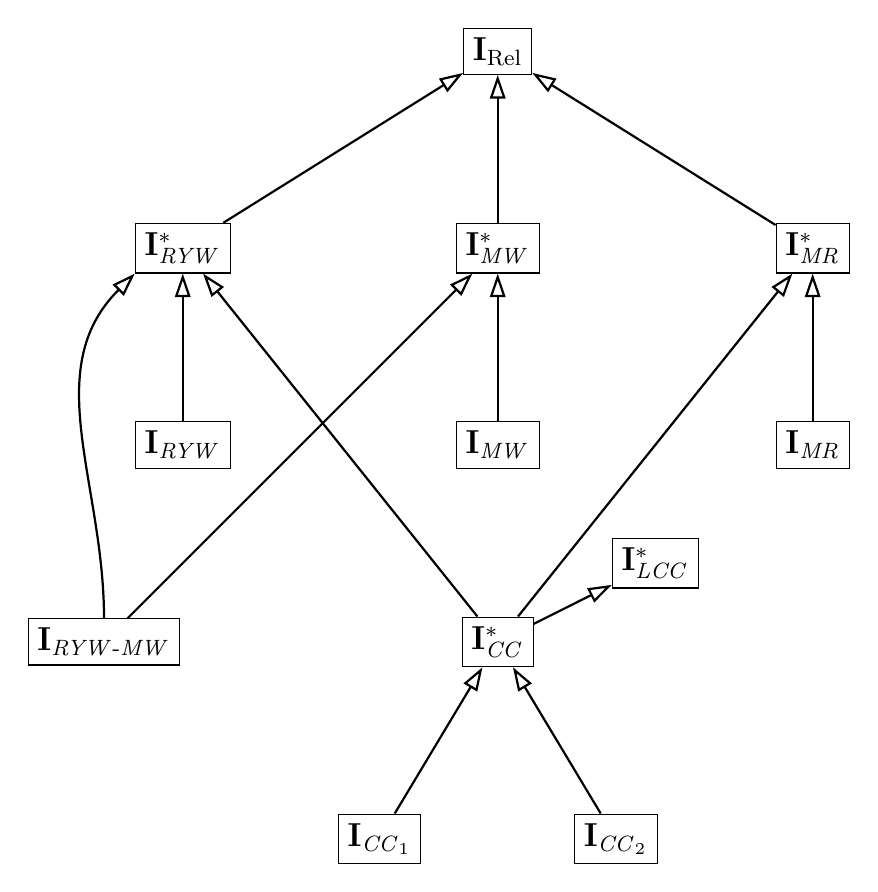
\begin{tikzpicture}[
    every node/.style={font=\large},
    arr/.style={-{Triangle[open, length=3mm]}, thick},
  ]

  % ── Nodes ────────────────────────────────────────────────────────────────

  % Bottom level
  \node[draw] (CC1)    at (-1.5, 0)  {$\mathbf{I}_{\CC_1}$};
  \node[draw] (CC2)    at ( 1.5, 0)  {$\mathbf{I}_{\CC_2}$};

  % Level 1
  \node[draw] (RYWMW)  at (-5,  2.5) {$\mathbf{I}_{\RYW\text{-}\MW}$};
  \node[draw] (CCstar) at ( 0,  2.5) {$\mathbf{I}_{\CC}^{*}$};

  % Level 2 (non-starred)
  \node[draw] (RYW)    at (-4, 5)    {$\mathbf{I}_{\RYW}$};
  \node[draw] (MW)     at ( 0, 5)    {$\mathbf{I}_{\MW}$};
  \node[draw] (MR)     at ( 4, 5)    {$\mathbf{I}_{\MR}$};
  \node[draw] (LCCstar) at ( 2, 3.5)   {$\mathbf{I}_{\LCC}^{*}$};

  % Level 3 (starred)
  \node[draw] (RYWstar) at (-4, 7.5) {$\mathbf{I}_{\RYW}^{*}$};
  \node[draw] (MWstar)  at ( 0, 7.5) {$\mathbf{I}_{\MW}^{*}$};
  \node[draw] (MRstar)  at ( 4, 7.5) {$\mathbf{I}_{\MR}^{*}$};

  % Level 4 (top)
  \node[draw] (Rel)     at ( 0, 10)  {$\mathbf{I}_{\mathrm{Rel}}$};

  % ── Edges ────────────────────────────────────────────────────────────────

  % CC1, CC2 → CC*
  \draw[arr] (CC1)     -- (CCstar);
  \draw[arr] (CC2)     -- (CCstar);

  % RYW-MW → RYW* (routed left of RYW to avoid overlap)
  \draw[arr] (RYWMW.north) to[out=90, in=225] (RYWstar.south west);

  % RYW-MW → MW*
  \draw[arr] (RYWMW)   -- (MWstar);

  % CC* → RYW*, MR*, LCC*
  \draw[arr] (CCstar)  -- (RYWstar);
  \draw[arr] (CCstar)  -- (MRstar);
  \draw[arr] (CCstar)  -- (LCCstar);

  % RYW → RYW*,  MW → MW*,  MR → MR*
  \draw[arr] (RYW)     -- (RYWstar);
  \draw[arr] (MW)      -- (MWstar);
  \draw[arr] (MR)      -- (MRstar);

  % RYW*, MW*, MR* → Rel
  \draw[arr] (RYWstar) -- (Rel);
  \draw[arr] (MWstar)  -- (Rel);
  \draw[arr] (MRstar)  -- (Rel);

  \end{tikzpicture}

  \vspace{0.5em}
  {\small
  \begin{tabular}{@{}ll@{}}
    $\mathbf{I}_{\mathrm{Rel}}$        & Relaxed Specification (Fig.~\ref{fig:relaxed-specification}) \\
    $\mathbf{I}_{\RYW}^{*}$           & Read Your Writes Specification (Fig.~\ref{fig:read-your-writes-spec}) \\
    $\mathbf{I}_{\RYW}$               & Read Your Writes Implementation (Fig.~\ref{fig:read-your-writes-impl}) \\
    $\mathbf{I}_{\MR}^{*}$            & Monotonic Reads Specification (Fig.~\ref{fig:monotonic-reads-spec}) \\
    $\mathbf{I}_{\MR}$                & Monotonic Reads Implementation (Fig.~\ref{fig:monotonic-reads-impl}) \\
    $\mathbf{I}_{\MW}^{*}$            & Monotonic Writes Specification (Fig.~\ref{fig:monotonic-writes-spec}) \\
    $\mathbf{I}_{\MW}$                & Monotonic Writes Implementation (Fig.~\ref{fig:monotonic-writes-impl}) \\
    $\mathbf{I}_{\RYW\text{-}\MW}$    & Read Your Writes and Monotonic Writes Implementation (Fig.~\ref{fig:ryw-mw-impl}) \\
    $\mathbf{I}_{\LCC}^{*}$           & Labeled Causal Consistency Spec (Fig.~\ref{fig:lcc-spec}) \\
    $\mathbf{I}_{\CC}^{*}$            & Causal Consistency Spec (Fig.~\ref{fig:causal-cons-spec}) \\
    $\mathbf{I}_{\CC_1}$              & Causal Consistency Implementation 1 (Fig.~\ref{fig:causal-map-95}) \\
    $\mathbf{I}_{\CC_2}$              & Causal Consistency Implementation 2 (Fig.~\ref{fig:LloydFreedman-protocol}) \\
  \end{tabular}
  }

  \caption{Refinement Hierarchy}
  \label{fig:refinement-hierarchy}
\end{figure}


\clearpage
\begin{figure}
\centering
\specfig{%
\begin{minipage}{0.90\linewidth}
   \figurealgtextsize
   \setlength{\abovedisplayskip}{0pt}%
   \setlength{\abovedisplayshortskip}{0pt}%
   \setlength{\belowdisplayskip}{0pt}%
   \setlength{\belowdisplayshortskip}{0pt}%
   \begin{mathpar}
   \begin{array}{|lr|}
      \hline
         𝐈_{\Rel} \ (\name{Relaxed Specification})
      & \\ \hline
         \CState ≔ \Unit
         & \bnote{Client State}
      \\
         \cInit(c) ≔ ⊥
         & \bnote{Client Initial State}
      \\
         \RState ≔ K ↦ V
         & \bnote{Replica State}
      \\
         \rInit(r, v₀) ≔ [\overline{ k ↦ v₀}]
         & \bnote{Replica Initial State}
      \\
      & \\
         \GetReqPayload ≔ \GetResPayload ≔ \Unit
         & \note{Get payload types}
      \\
         \getReq \ (\_) (\_, σ)  ≔ 
         & \note{At client: } \bnote{Get Request}
      \\ \t
         \ret〈○, p〉
         & \note{No payload}
      \\
         \getGuard \ (\_) (\_) (\_, \_, \_) ≔
         & \note{At replica: } \bnote{Get Guard}
      \\ \t
         \ret \true
         & \note{}
      \\
         \get \ (k) (\_) (\_, \_, ς)  ≔
         & \note{At replica: } \bnote{Get}
      \\ \t
         \llet〈v, \_〉← ς (k)
         & \note{}
      \\ \t
         \ret〈 v, ○, ς 〉
         & \note{No payload}
      \\
         \getRes \ (\_, \_) (\_) (\_, σ) ≔
         & \note{At client: } \bnote{Get Response}
      \\ \t
         \ret σ
         & \note{}
      \\
      & \\
         \PutReqPayload ≔ \Unit
         & \note{Put payload types} 
      \\
         \putReq \ (k, \_) (\_, σ) ≔ 
         & \note{At client: }\bnote{Put Request}
      \\ \t
         \ret〈○, σ〉
         & \note{No payload}
      \\
         \putGuard \ (\_, \_) (\_) (\_, \_, \_) ≔ 
         & \note{At replica: } \bnote{Put Guard}
      \\ \t
         \ret \true
         & \note{}          
      \\
         \lput \ (k, v) (\_) (\_, \_, ς) ≔ 
         & \note{At replica: } \bnote{Put}
      \\ \t
         \ret ς [k ↦ v]
      & \\ \hline
   \end{array}
   \end{mathpar}
\end{minipage}%
}
   \caption{Relaxed Specification}
   \label{fig:relaxed-specification}
\end{figure}
